\chapter{Réalisation et résultats}

\section{Introduction}

Après avoir achevé l’étape d’analyse et conception de l’application, on va entamer dans ce chapitre la partie réalisation et implémentation dans laquelle on va s’assurer que le système est prêt pour être exploité par les utilisateurs finaux.


\section{Choix des technologies}

\subsection{UML}

Le Langage de Modélisation Unifié, de l'anglais Unified Modeling Language (UML), est un langage de modélisation graphique à base de pictogrammes conçu comme une méthode normalisée de visualisation dans les domaines du développement logiciel et en conception orientée objet.

\begin{figure}[!h]
\begin{center}

\includegraphics[height=8cm]{UML.svg.png}
\end{center}
\caption{UML}
\end{figure}


\subsection{Next js}

Next.js est un cadriciel (framework) gratuit et open source s'appuyant sur la librairie JavaScript React et sur la technologie Node.js.

Le framework permet de créer des applications web universelles ou parfois appelées isomorphiques, signifiant que le code source est partagé entre le client et le serveur, de même que le font ses concurrents (Gatsby, Nuxt.js, Blitz).

\begin{figure}[!h]
\begin{center}

\includegraphics[height=8cm]{Nextjs.svg.png}
\end{center}
\caption{NEXT.JS}
\end{figure}

\subsection{Postgresql}

PostgreSQL est un système de gestion de base de données relationnelle orienté objet puissant et open source qui est capable de prendre en charge en toute sécurité les charges de travail de données les plus complexes. Alors que MySQL donne la priorité à l'évolutivité et aux performances, Postgres donne la priorité à la conformité et à l'extensibilité SQL.

\begin{figure}[!h]
\begin{center}

\includegraphics[height=8cm]{Postgresql.svg.png}
\end{center}
\caption{Postgresql}
\end{figure}



\subsection{Cassandra}

Apache Cassandra est un système de gestion de base de données (SGBD) de type NoSQL conçu pour gérer des quantités massives de données sur un grand nombre de serveurs, assurant une haute disponibilité en éliminant les points de défaillance unique. Il permet une répartition robuste sur plusieurs centres de données 3, avec une réplication asynchrone sans nœud maître et une faible latence pour les opérations de tous les clients.

\begin{figure}[!h]
\begin{center}

\includegraphics[height=6cm]{Cassandra.svg.png}
\end{center}
\caption{Cassandra}
\end{figure}

\subsection{Latex}

LaTeX (dont le logo est \LaTeX) est un langage et un système de composition de documents. Il s'agit d'une collection de macro-commandes destinées à faciliter l'utilisation du « processeur de texte » TeX de Donald Knuth.

LaTeX permet de rédiger des documents dont la mise en page est réalisée automatiquement en se conformant du mieux possible à des normes typographiques. Une fonctionnalité distinctive de LaTeX est son mode mathématique, qui permet de composer des formules complexes.

\begin{figure}[!h]
\begin{center}

\includegraphics[height=6cm]{LaTeX.svg.png}
\end{center}
\caption{\LaTeX}
\end{figure}

\subsection{Visual Studio Code}

Visual Studio Code est un éditeur de code extensible développé par Microsoft pour Windows, Linux et macOS.

Les fonctionnalités incluent la prise en charge du débogage, la mise en évidence de la syntaxe, la complétion intelligente du code, les snippets, la refactorisation du code et Git intégré. Les utilisateurs peuvent modifier le thème, les raccourcis clavier, les préférences et installer des extensions qui ajoutent des fonctionnalités supplémentaires.

\begin{figure}[!h]
\begin{center}

\includegraphics[height=6cm]{vscode.svg.png}
\end{center}
\caption{vscode}
\end{figure}


\section{Interfaces graphiques}

\subsection{Page de login}

Page de login 

\begin{figure}[!h]
\begin{center}
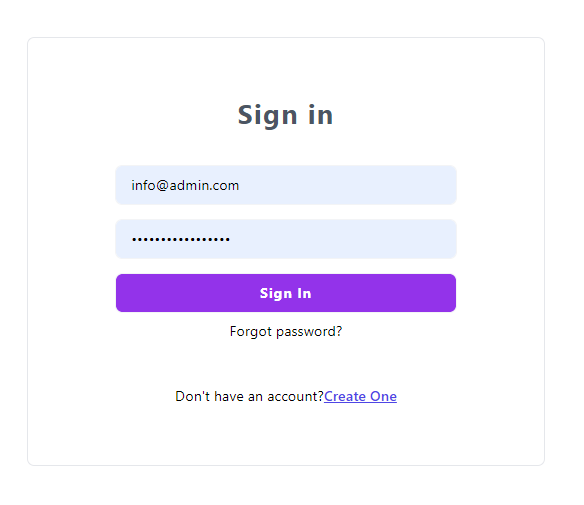
\includegraphics[height=10cm]{log.png}
\end{center}
\caption{Page de login }
\end{figure}


\subsection{Profile du patient}

le profile du patient contient ses informations personnelles.

\begin{figure}[!h]
\centering
\begin{center}
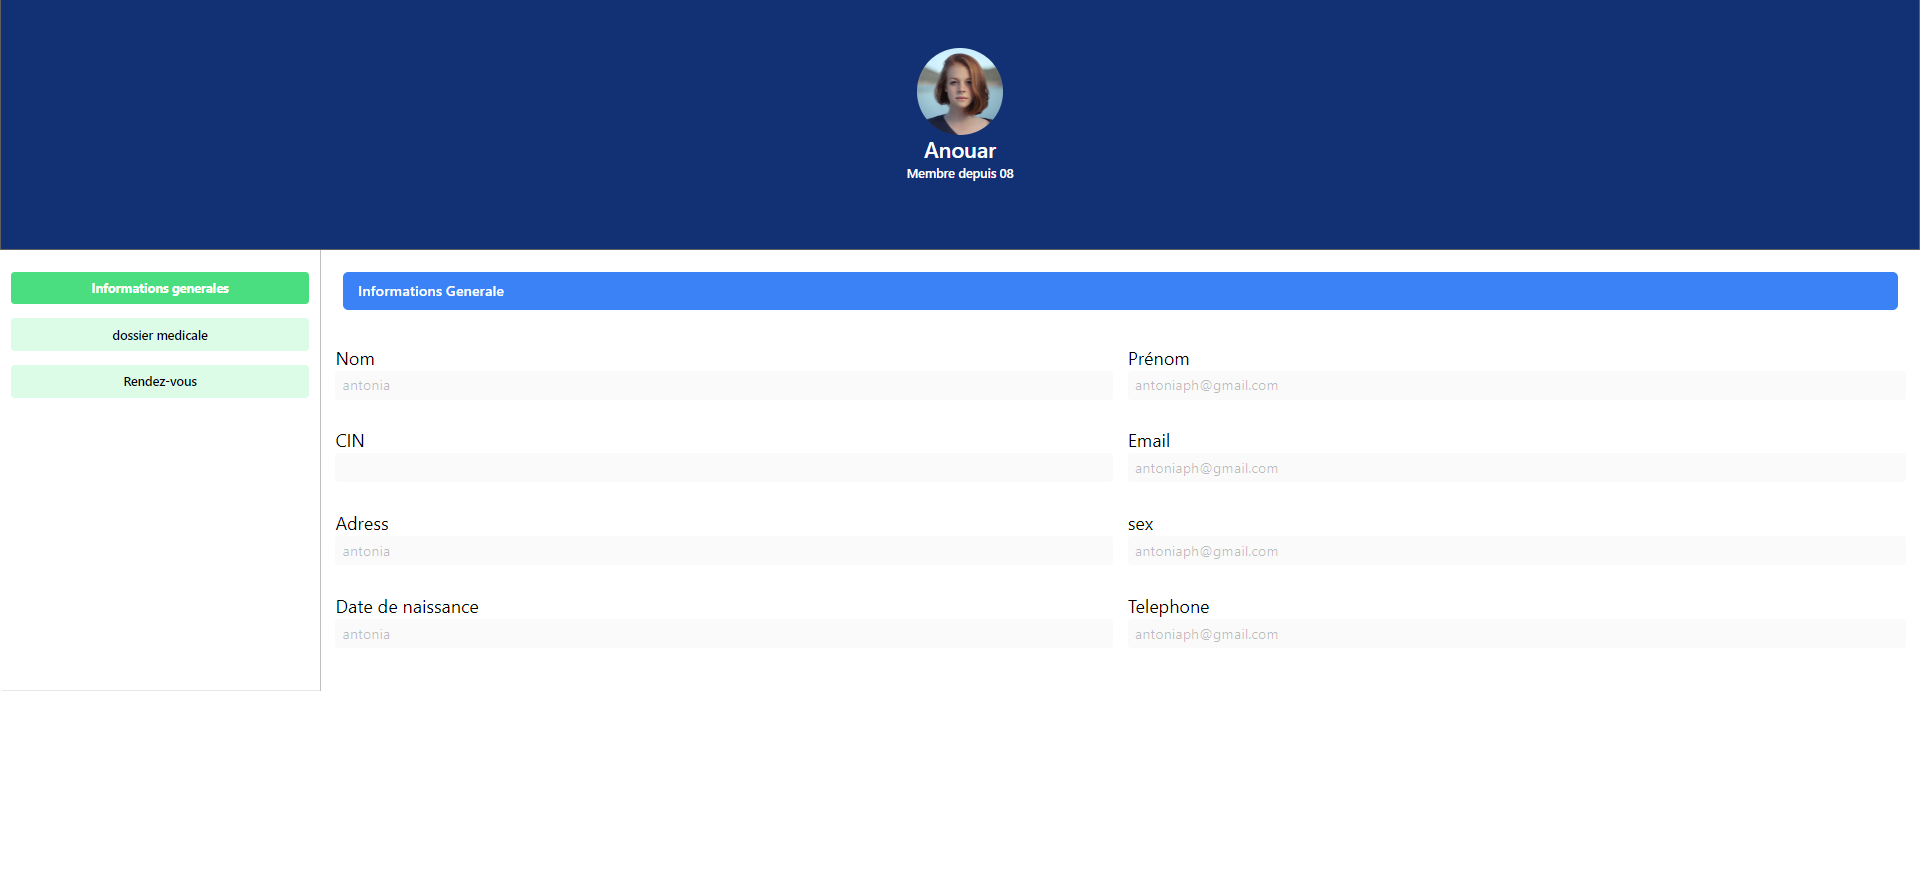
\includegraphics[height=10cm,width=18cm]{gen.png}
\end{center}
\caption{Profile du patient}
\end{figure}


\subsection{Dossier medical du patient}

Le dossier médical du patient contient les dernières actions faites par le patients

\begin{figure}[!h]
\begin{center}
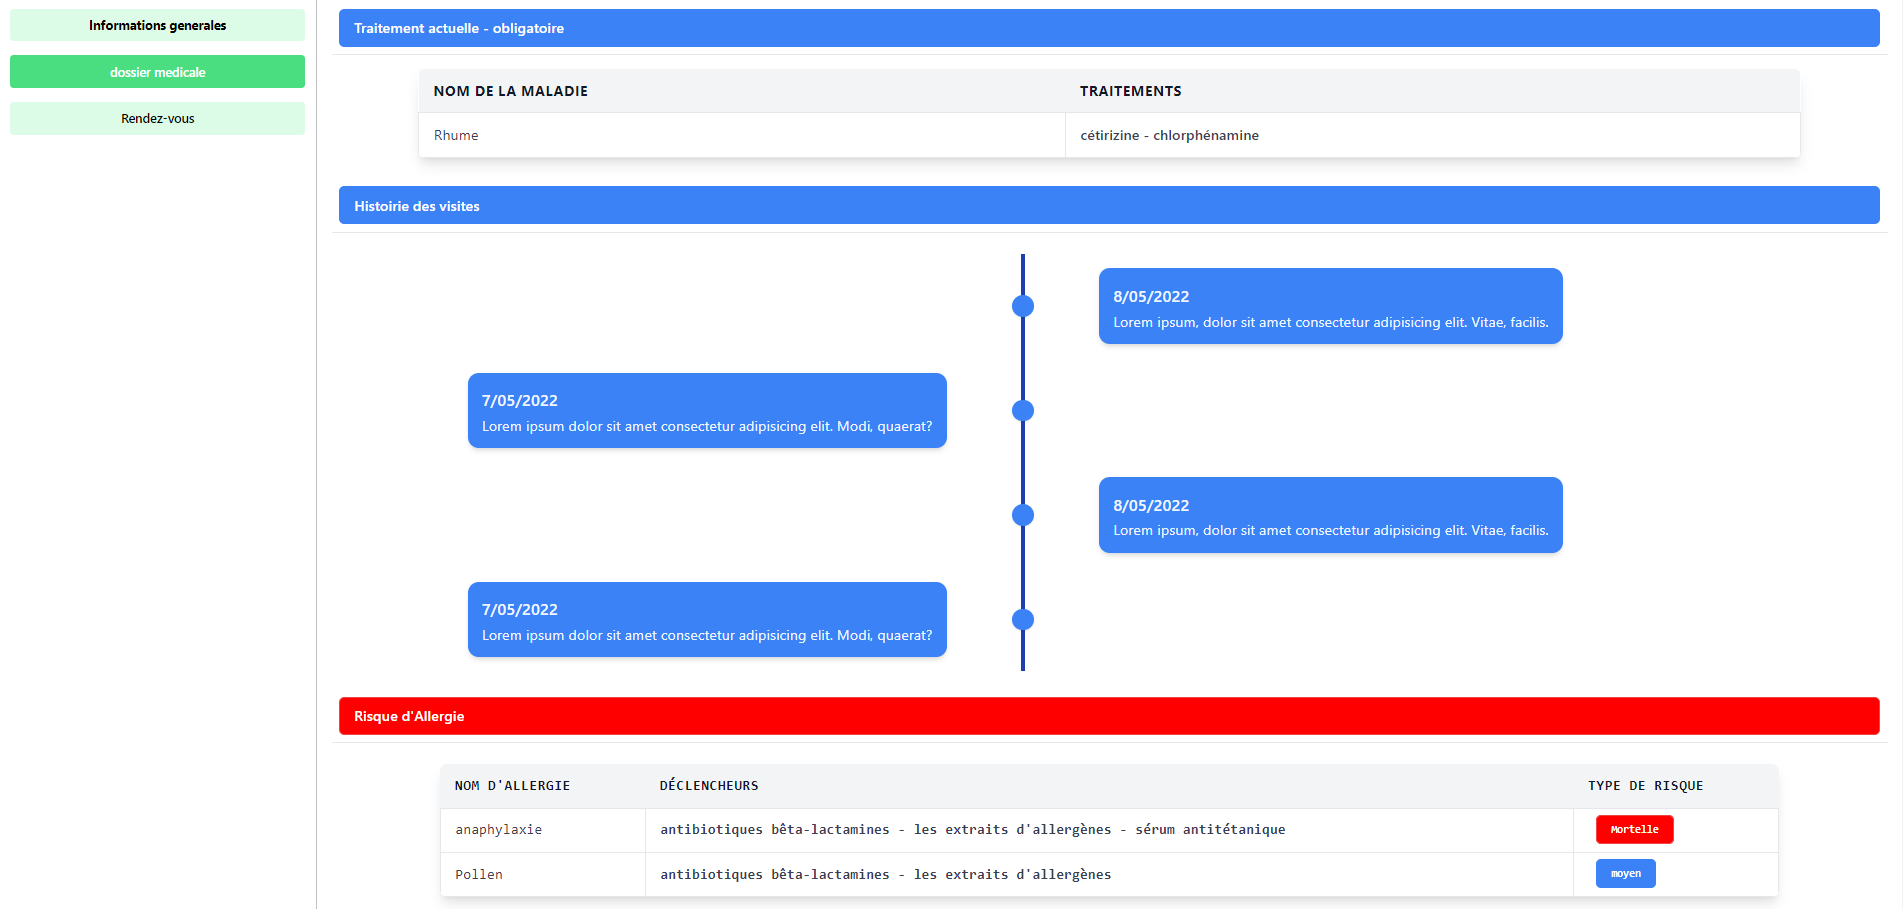
\includegraphics[height=8cm,width=18cm]{med.png}
\end{center}
\caption{Dossier medical du patient}
\end{figure}










\section{Conclusion}